\documentclass[t, 				             
			   final,
			   12pt, 				         
			   xcolor={usenames,dvipsnames}, 
			   table]{beamer}

% pacotes utilizados.
\usepackage[alf]{abntex2cite}
\usepackage{amsmath}
\usepackage[brazil]{babel}
\usepackage{booktabs}
\usepackage{caption}
\usepackage{ctable}
\usepackage[utf8]{inputenc}
\usepackage{listings}
\usepackage{multicol}
\usepackage{multirow}
\usepackage{todo}


% configuração do tema
\usetheme[pageofpages=de,
          bullet=square,			
          titleline=true,				
          alternativetitlepage=true,			
          titlepagelogo=imagens/logo-puc,	
          watermarkheight=70px,		
          watermarkheightmult=4	
          ]{Torino}

\setbeamertemplate{sections/subsections in toc}[square]
\setbeamertemplate{bibliography item}[default]

\usecolortheme{freewilly}

% Block Environment
% -------------------------------
\setbeamertemplate {blocks}[default]
\setbeamercolor{block title}{fg=red!0!green!15!blue!85!, bg=red!33!green!37!blue!15!}
\setbeamercolor{block body}{fg=black, bg=red!32!green!33!blue!5}
\setbeamercolor{block title alerted}{fg=white, bg=red!40!black}
\setbeamercolor{block body alerted}{fg=black, bg=red!5!white}
\setbeamercolor{block title example}{fg=white, bg=green!40!black}
\setbeamercolor{block body example}{fg=black, bg=green!5!white}
\setbeamerfont{block title}{size=\scriptsize, series=\bfseries}


\definecolor{javared}{rgb}{0.6,0,0} % for strings
\definecolor{javagreen}{rgb}{0.25,0.5,0.35} % comments
\definecolor{javapurple}{rgb}{0.5,0,0.35} % keywords
\definecolor{javadocblue}{rgb}{0.25,0.35,0.75} % javadoc
 
\lstset{}

\lstdefinestyle{BashInputBasicStyle}{
	language=bash,
	basicstyle=\normalsize\ttfamily,
	columns=fullflexible,
	tabsize=2,
	showstringspaces=false,
	frame=single,
	inputencoding=utf8,
	rulecolor=\color{gray}
}

\lstdefinestyle{BashInputStyle}{
  language=bash,
  basicstyle=\normalsize\ttfamily,
  numbers=left,
  numberstyle=\tiny,
  numbersep=2pt,
  frame=tb,
  columns=fullflexible,
  tabsize=2,
  showstringspaces=false,
  commentstyle=\color{gray},
  inputencoding=utf8,
  rulecolor=\color{gray}
}

\lstdefinestyle{RubyInputStyle}{
    language=ruby,
    basicstyle=\scriptsize\ttfamily,
    keywordstyle=\color{javapurple},
    identifierstyle=\color{black},
    commentstyle=\color{javagreen},
	stringstyle=\color{blue},
    showstringspaces=false,
    numbers=left,
    numberstyle=\color{gray}\tiny,
    tabsize=3,
    extendedchars=\true,
    inputencoding=utf8,
%   frame=single, 
    columns=fixed,
    backgroundcolor=\color{red!32!green!33!blue!5}
}    
%  language=ruby,
%  basicstyle=\normalsize\ttfamily,
%  keywordstyle=\color{OrangeRed},
%  identifierstyle=\color{Turquoise},
%  commentstyle=\color{gray},
%  stringstyle=\color{YellowOrange},
%  numbers=left,
%  numberstyle=\tiny,
%  numbersep=2pt,
%  frame=tb,
%  columns=fullflexible,
%  backgroundcolor=\color{white!80},
%  linewidth=0.9\linewidth,
%  tabsize=2,
%  showstringspaces=false
%  inputencoding=utf8


\lstdefinestyle{JavaInputStyle}{
	language=Java,
	basicstyle=\ttfamily,
	keywordstyle=\color{javapurple}\bfseries,
	stringstyle=\color{javared},
	commentstyle=\color{javagreen},
	morecomment=[s][\color{javadocblue}]{/**}{*/},
	numbers=left,
	numberstyle=\tiny\color{black},
	numbersep=10pt,
	tabsize=2,
	showspaces=false,
	showstringspaces=false,
	frame=tb,
	columns=fullflexible,
	backgroundcolor=\color{white!80},
	linewidth=0.9\linewidth,
	inputencoding=utf8
}

\begin{document}
	\author{Luiz Alberto Ferreira Gomes}
\title{Linguagem Ruby}
\subtitle{Seminários da Computação}
\institute{Curso de Ciência da Computação}
\date{\today}

	\begin{frame}[plain]
  \titlepage
\end{frame}
	\AtBeginSection[]
{
  \begin{frame}{Ruby}
    \tableofcontents[currentsection]
  \end{frame}
}
  
	\section{Introdução}	
	%-------------------------------------------------------------------------------------- Início
\begin{frame}[fragile,t]{Ruby}
  \begin{itemize}
    \item Linguagem inventada por Yukihiro "Matz" Matsumoto
    \item Versão 1.0 liberada em 1996(Japão)
    \item Popularizado no início de 2005 pelo Rails
  \end{itemize}   
  \begin{figure}[hbt]
    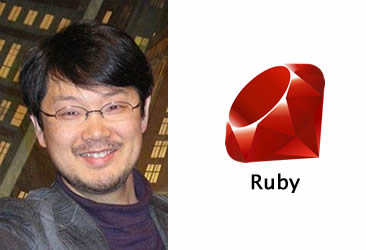
\includegraphics[scale=.5]{imagens/matz.jpg}
  \end{figure}
\end{frame}
%-------------------------------------------------------------------------------------- Início
\begin{frame}[fragile,t]{Ruby}
  \begin{itemize}
    \item Linguagem \alert{dinâmica} e \alert{orientada a objetos}
    \item Elegante, \alert{expressiva} e declarativa
    \item Influenciada pelo Perl, Smalltalk, Eiffel e Lisp
  \end{itemize}   
\end{frame}
%-------------------------------------------------------------------------------------- Início
\begin{frame}[fragile,t]{..Java..}
  \begin{lstlisting}[style=JavaInputStyle]
    public class Print3Times {
      public static void main(String[] args) {
        for(int i = 0; i < 3; i++) {
          System.out.println("Hello World!")
        }
      }
    }
  \end{lstlisting}
\end{frame}
%-------------------------------------------------------------------------------------- Início
\begin{frame}[fragile,t]{..Ruby..}
		\lstinputlisting[style=RubyInputStyle, caption=hello.rb]{codigos/ruby/01-ruby-introducao/hello.rb}
\end{frame}
%-------------------------------------------------------------------------------------- Início
\begin{frame}[fragile,t]{Básico do Ruby}
  \begin{itemize}
    \item Indentação de 2 espaços para cada nível aninhado (\alert{recomendado})
    \item \# é utilizado para comentários
    \begin{itemize}
    	\item use com moderação, o código deve ser auto documentado
    \end{itemize}
    \item Scripts utilizam a extensão \verb!.rb! 
		\lstinputlisting[style=RubyInputStyle, caption=hello.rb]{codigos/ruby/01-ruby-introducao/hello.rb}
  \end{itemize}   
\end{frame}
%-------------------------------------------------------------------------------------- Início
\begin{frame}[fragile,t]{Saída na Tela}
  \begin{itemize}
    \item \verb!puts! é método \alert{padrão} para impressão em tela 
    \begin{itemize}
    	\item insere uma quebra de linha após a impressão
    	\item similar ao \verb!System.out.println! do Java
    \end{itemize}
    \item \alert{p} é utilizado para depuração
  \end{itemize}   
\end{frame}
%-------------------------------------------------------------------------------------- Início
\begin{frame}[fragile,t]{Entrada pelo Teclado}
  \begin{itemize}
    \item \verb!gets! é método padrão para receber um valor pelo teclado 
		\begin{lstlisting}[style=RubyInputStyle]
# recebe um valor do tipo string.
nome = gets
  	\end{lstlisting}
    \item Utilize \verb!gets.chomp! para remover o caracter de nova linha.
		\begin{lstlisting}[style=RubyInputStyle]
# remove o caracter de nova linha.
nome = gets.chomp
  	\end{lstlisting}
  	\item Utilize \verb!gets.chomp.to_i! para converter o valor lido para inteiro. 
		\begin{lstlisting}[style=RubyInputStyle]
# converte a string recebida para inteiro.
nome = gets.chomp.to_i
  	\end{lstlisting}
  \end{itemize}   
\end{frame}
%-------------------------------------------------------------------------------------- Início
\begin{frame}[fragile,t]{Convenção de Nomes}
  \begin{itemize}
    \item Variáveis e Métodos
    \begin{itemize}
    	\item em minúsculas e \verb!separada_por_sublinhado! (tenha mais de uma palavra)
    	\item métodos ainda permitem no final os caracteres \verb|?!|
    \end{itemize}
    \item Constantes
    \begin{itemize}
    	\item tanto \verb!TODAS_AS_LETRAS_EM_MAIUSCULAS! ou no formato \verb!CamelCase!
    \end{itemize}
    \item Classes(e módulos)
    \begin{itemize}
    	\item formato \verb!CamelCase! 
    \end{itemize}
  \end{itemize}
\end{frame}
%-------------------------------------------------------------------------------------- Início
\begin{frame}[fragile,t]{Remoção do Ponto-e-Vírgula}
  \begin{itemize}
    \item Não coloque o ponto-e-vírgula no final da linha
    \item Pode ser utilizado para colocar várias declarações em uma linha
    \begin{itemize}
      \item altamente desencorajado
    \end{itemize}
    \begin{lstlisting}[style=RubyInputStyle]
a = 3	
a = 3; b = 5 
    \end{lstlisting}
  \end{itemize}
\end{frame}
%-------------------------------------------------------------------------------------- Início
\begin{frame}[allowframebreaks, fragile,t]{Interactive Ruby (IRB)}
  \begin{itemize}
    \item Console \alert{interativa} para interpretação de comandos Ruby
    \item Instalado com o interpretador Ruby
    \item Permite a \alert{execução} de comandos rapidamente
  \end{itemize}
  \begin{figure}[hbt]
    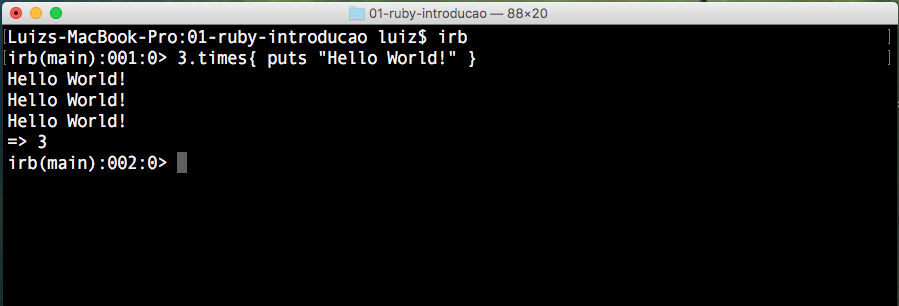
\includegraphics[scale=.35]{imagens/ruby-irb.png}
  \end{figure}
\framebreak
  \begin{itemize}
  	\item Permite a \alert{execução} de \alert{scripts} contendo vários comandos
  \end{itemize}
  \begin{figure}[hbt]
    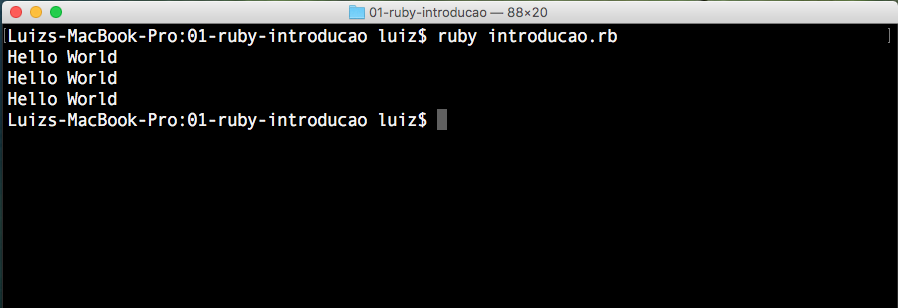
\includegraphics[scale=.35]{imagens/ruby-interpretador.png}
  \end{figure}
\end{frame}
%-------------------------------------------------------------------------------------- Início
\begin{frame}[allowframebreaks,fragile,t]{Exercícios}
  \begin{itemize}
    \item Escreva um script Ruby para imprimir um nome lido teclado 5 vezes.
  \end{itemize}
\framebreak
  \begin{itemize}
    \item \textbf{Solução}:
  \end{itemize}	
  \begin{lstlisting}[style=RubyInputStyle]
nome = gets.chomp
5.times { puts nome }
  \end{lstlisting}
\end{frame}

	\section{Entrada e Saída}
	%-------------------------------------------------------------------------------------- Início
\begin{frame}[fragile,t]{Entrada pelo Teclado}
    \begin{itemize}
      \item \verb!gets! é método \alert{padrão para receber} um valor pelo teclado 
          \begin{lstlisting}[style=RubyInputStyle]
  # recebe um valor do tipo string.
  nome = gets
        \end{lstlisting}
      \item Utilize \verb!gets.chomp! para remover o caracter de nova linha.
          \begin{lstlisting}[style=RubyInputStyle]
  # remove o caracter de nova linha.
  nome = gets.chomp
        \end{lstlisting}
        \item Utilize \verb!gets.chomp.to_i! para converter o valor lido para inteiro. 
          \begin{lstlisting}[style=RubyInputStyle]
  # converte a string recebida para inteiro.
  idade = gets.chomp.to_i
        \end{lstlisting}
    \end{itemize}   
  \end{frame}
%-------------------------------------------------------------------------------------- Início
\begin{frame}[fragile,t]{Saída na Tela}
    \begin{itemize}
      \item \verb!puts! é método \alert{padrão} para impressão em tela 
      \begin{itemize}
          \item insere uma quebra de linha após a impressão
          \item similar ao \verb!System.out.println! do Java
      \end{itemize}
      \begin{lstlisting}[style=RubyInputStyle]
# exibe da tela do computador.
puts "Informacoes do jogador"
puts "Nome  %s" % nome 
puts "Idade %d" % idade
puts "Nome %s \nIdade %d" % [nome, idade]
      \end{lstlisting}
    \end{itemize}   
  \end{frame}
  
	\section{Controle de Fluxo}
	%-------------------------------------------------------------------------------------- Início
\begin{frame}[allowframebreaks, fragile,c]{Controle de Fluxo}
  \begin{center}
    \Large \verb!if ... elsif ... else! \\ \verb!case! \\ \verb!unless!
  \end{center}   
\framebreak
  \begin{itemize}
    \item \alert{Não} existe a necessidade de uso de \alert{parênteses} ou \alert{chaves}
    \item \alert{Utilize} a instrução \verb!end! no final do bloco
  \end{itemize}   
  \begin{columns}
    \begin{column}{0.5\textwidth}
    		\lstinputlisting[style=RubyInputStyle, caption=if.rb]{codigos/ruby/02-fluxo-de-controle/if.rb}  
    \end{column}
    \begin{column}{0.5\textwidth}
    		\lstinputlisting[style=RubyInputStyle, caption=unless.rb]{codigos/ruby/02-fluxo-de-controle/unless.rb}  
    \end{column}
  \end{columns}
\framebreak
    		\lstinputlisting[style=RubyInputStyle, caption=case\_1.rb]{codigos/ruby/02-fluxo-de-controle/case_1.rb}  
\framebreak
    		\lstinputlisting[style=RubyInputStyle, caption=case\_2.rb]{codigos/ruby/02-fluxo-de-controle/case_2.rb}  
\end{frame}
%-------------------------------------------------------------------------------------- Início
\begin{frame}[fragile,t]{Operadores Lógicos (em ordem de precedência)}
	\begin{table}[tp] 	
		\setlength{\tabcolsep}{8pt}
    \setlength{\extrarowheight}{2pt}    
		\begin{tabular}{p{2.5cm}l}
    	\toprule
      $<=, <, >, >=$ &  Comparação\\
      $==, !=$ & Igual ou diferente  \\
      $\&\&$ &  Conectivo \textbf{e} \\
      $||$ & Conectivo \textbf{ou} \\
	    \bottomrule
		\end{tabular}
	\end{table}   
\end{frame}
%-------------------------------------------------------------------------------------- Início
\begin{frame}[fragile,t]{True e False}
  \begin{itemize}
    \item \alert{false} e \alert{nil} são booleanos \alert{FALSOS}
    \item Todo o restante é \alert{VERDADEIRO}
	\lstinputlisting[style=RubyInputStyle, caption=true\_false.rb]{codigos/ruby/02-fluxo-de-controle/true_false.rb}
  \end{itemize}   
\end{frame}
%-------------------------------------------------------------------------------------- Início
\begin{frame}[fragile,t]{Exercícios}
  \begin{enumerate}
    \item Digite as seguintes expressões no IRB e verifique os resultados.
  \end{enumerate}
	\begin{lstlisting}[style=RubyInputStyle]
		(32 * 4) >= 129
		false != !true
		true == 4
		false == (847 == '847')
		(!true || (!(100 / 5) == 20) || ((328 / 4) == 82) || false 
	\end{lstlisting}
\end{frame}
%-------------------------------------------------------------------------------------- Início
\begin{frame}[fragile,t]{Recapitulando}
  \begin{itemize}
    \item Existe muitas opções de fluxo de controle
    \item A formato em um linha é muito expressiva
    \item Exceto \verb!nil! e \verb!false!, os demais valores são verdadeiros.
  \end{itemize}
\end{frame}




	\section{Loops e Interações}	
	
\begin{frame}[allowframebreaks, fragile,t]{Loops e Interações}
  \begin{center}
    \Large \verb!loop! \\ \verb!while e until! \\ \verb!for! \\ \verb!each e times!
  \end{center}   
\framebreak

  \begin{itemize}
	\item \verb!loop!
  \end{itemize}
  \lstinputlisting[style=RubyInputStyle, caption=loop.rb]{codigos/ruby/03-loop-e-interacoes/loop.rb}

\framebreak
  \begin{itemize}
	\item \verb!while e until!
  \end{itemize}
     
  \begin{columns}
    \begin{column}{0.5\textwidth}
  \lstinputlisting[style=RubyInputStyle, caption=while.rb]{codigos/ruby/03-loop-e-interacoes/while.rb}
    \end{column}
    \begin{column}{0.5\textwidth}  %%<--- here
  \lstinputlisting[style=RubyInputStyle, caption=until.rb]{codigos/ruby/03-loop-e-interacoes/until.rb}
    \end{column}
  \end{columns}

\framebreak
  \begin{itemize}
		\item \verb!for! (\alert{dificilmente empregado})
    \item \verb!each/times! é preferível
  \end{itemize}
  
  \lstinputlisting[style=RubyInputStyle, caption=for\_loop.rb]{codigos/ruby/03-loop-e-interacoes/for_loop.rb}

\framebreak
  \begin{itemize}
	\item \verb!each!
  \end{itemize}
     
  \begin{columns}
    \begin{column}{0.5\textwidth}
  \lstinputlisting[style=RubyInputStyle, caption=each\_1.rb]{codigos/ruby/03-loop-e-interacoes/each_1.rb}  
    \end{column}
    \begin{column}{0.5\textwidth} 
  \lstinputlisting[style=RubyInputStyle, caption=each\_2.rb]{codigos/ruby/03-loop-e-interacoes/each_2.rb}

    \end{column}
  \end{columns}
\end{frame}
\begin{frame}[allowframebreaks,fragile,t]{Hora de Colocar as Mão na Massa}
  \begin{enumerate}
    \item Escreva um \textit{script} Ruby leia o nome de um jogador do jogo de adivinha e 
      apresente o valor lido.
    \item O \textit{script} Ruby deverá sortear um número de 1 a 10 e permite que 
    o usuário tente 3 vezes até acertá-lo. A cada tentativa errada, o programa informa
    se o número a adivinhar está abaixo ou acima. \textbf{Dica:} utilize rand(n) + 1 
  \end{enumerate}
  \framebreak
\end{frame}
%-------------------------------------------------------------------------------------- Início
\begin{frame}[allowframebreaks,fragile,t]{Solução do Exercício}
  \lstinputlisting[style=RubyInputStyle, caption=loop.rb]{codigos/ruby/03-loop-e-interacoes/jogo-de-adivinha.rb}
\end{frame}

\begin{frame}[fragile,t]{Recapitulando}
  \begin{itemize}
    \item Existe muitas opções de loops e interações
    \item \verb!each! é \alert{preferível} ao loop \verb!for! para percorrer arrays
  \end{itemize}
\end{frame}




	%\section{Funções e Métodos}
	%
\begin{frame}[fragile,t]{Funções e Métodos}
  \begin{itemize}
    \item Tecnicamente, uma \alert{função} é definida \alert{fora} de uma classe
    \item Um \alert{método} é definido dentro de uma classe
    \item Em Ruby, \alert{toda} função/método é pertence a pelo menos uma classe
    \begin{itemize}
      \item nem sempre explicitamente escrito em uma classe
    \end{itemize}
  \end{itemize}
  \framebreak   
  \begin{center}
    Conclusão: Toda \alert{função} é na verdade um \alert{método} em Ruby  
  \end{center}
\end{frame}

\begin{frame}[fragile,t]{Métodos}
  \begin{itemize}
    \item Parênteses são \alert{opcionais}
    \begin{itemize}
      \item tanto para definição quanto para a chamada do método
    \end{itemize}
    \item Usado para tornar o código mais claro
  \end{itemize}
  \begin{block}{parens.rb}
  	\lstinputlisting[style=RubyInputStyle]{codigos/ruby/04-funcoes-e-metodos/parens.rb}
  \end{block}
  
    
\end{frame}

\begin{frame}[fragile,t]{Parâmetros e Retorno}
  \begin{itemize}
    \item Não é necessário declarar o tipo dos parâmetros
    \item O método pode retornar qualquer valor
    \item O comando \verb!return! é opcional
    \begin{itemize}
      \item o valor da \alert{última linha} executada é retornada 
    \end{itemize}
  \end{itemize}
  
  \lstinputlisting[style=RubyInputStyle, caption=return\_optional.rb]{codigos/ruby/04-funcoes-e-metodos/return_optional.rb}
    
\end{frame}

\begin{frame}[fragile,t]{Nomes de Métodos Expressivos}
  \begin{itemize}
    \item Nomes de métodos podem terminar com:
    \begin{itemize}
    	\item \alert{'?'} - métodos com retorno booleano
    	\item \alert{'!'} - métodos com efeitos colaterais
    \end{itemize}
    
	\lstinputlisting[style=RubyInputStyle, caption=expressive.rb]{codigos/ruby/04-funcoes-e-metodos/expressive.rb}
  \end{itemize}   
\end{frame}

\begin{frame}[fragile,t]{Argumentos Padrões(Defaults)}
  \begin{itemize}
    \item Métodos podem ter argumentos padrões
    \begin{itemize}
    	\item se o valor é passado, ele é utilizado
    	\item senão, o valor padrão é utilizado
    \end{itemize}
  \end{itemize}  
  \lstinputlisting[style=RubyInputStyle, caption=default\_args.rb]{codigos/ruby/04-funcoes-e-metodos/default_args.rb}
\end{frame}

\begin{frame}[fragile,t]{Quantidade Variável de Argumentos}
  \begin{itemize}
    \item \alert{*} prefixa o parâmetro com quantidade variável de argumentos
  \end{itemize}
  \begin{itemize}
    \item Pode ser utilizado com parâmetros no início, meio e final
  \end{itemize}
  \lstinputlisting[style=RubyInputStyle, caption=splat.rb]{codigos/ruby/04-funcoes-e-metodos/splat.rb}
\end{frame}
%-------------------------------------------------------------------------------------- Início
\begin{frame}[fragile,t]{Exercícios}
  \begin{enumerate}
    \item Escreva uma função que receba como parâmetro um custo retorna a taxa de entrega
		de acordo com a seguinte regra:
		\begin{itemize}
			\item a taxa de entrega será igual a 10.00 se o custo for menor do que 25.00;
			\item a taxa será igual a 20.00 se o custo for menor do que 100.00;
			\item a taxa a taxa será igual a 30.00 se o custo for menor do que 200.00;
			\item a taxa será igual a 35.00 se o custo for maior ou igual do que 200.00;
		\end{itemize} 
  \end{enumerate}
\end{frame}

\begin{frame}[fragile,t]{Recapitulando}
  \begin{itemize}
    \item \alert{Não há necessidade} de declarar o tipo de parâmetro passado ou retornado (linguagem dinâmica)
    \item \verb!return! é \alert{opcional} - a última linha executável é "retornada"
    \item Permite métodos com \alert{quantidade variável} de argumentos ou argumentos padrão
  \end{itemize}
\end{frame}




	%%%-------------------------------------------------------------------------------------- Início
\begin{frame}[fragile,t]{Para Saber Mais}
  \begin{itemize}
    \item \url{https://www.ruby-lang.org/en/}
    \begin{itemize}
     \item referência oficial da linguagem Ruby onde a toda a sua documentação está disponível
	para ser consultada.
    \end{itemize}

    \item \url{http://rubyonrails.org/}
    \begin{itemize}
     \item referência oficial do framework Rails onde a toda a sua documentação está disponível
	para ser consultada.
    \end{itemize}
    
    \item \url{http://www.codecademy.com/pt/tracks/ruby}
    \begin{itemize}
     \item interessante curso iterativo em portugês sobre a linguagem Ruby.
    \end{itemize}

  \end{itemize}
  
  
\end{frame}
\end{document}
